% ==============================================================
% BAREBONE LATEX TEMPLATE
% Based on: protocol_documentation.tex style
% ==============================================================

\documentclass[11pt,a4paper]{article}

% ============================================================
% PACKAGES
% ============================================================
\usepackage[utf8]{inputenc}
\usepackage[T1]{fontenc}
\usepackage{lmodern}
\usepackage[margin=1in]{geometry}
\usepackage{graphicx}
\usepackage{hyperref}
\usepackage{xcolor}
\usepackage{listings}
\usepackage{booktabs}
\usepackage{tabularx}
\usepackage{longtable}
\usepackage{amsmath}
\usepackage{amssymb}
\usepackage{bytefield}
\usepackage{fancyhdr}
\usepackage{titlesec}
\usepackage{enumitem}
\usepackage{tcolorbox}
\usepackage{float}
\usepackage{caption}
\usepackage{subcaption}
\usepackage{multicol}
\usepackage{tikz}
\usetikzlibrary{shapes,arrows,positioning,calc}

% ============================================================
% COLOR DEFINITIONS
% ============================================================
\definecolor{skyblue}{RGB}{0,102,204}
\definecolor{darkblue}{RGB}{0,51,102}
\definecolor{codebg}{RGB}{245,245,245}
\definecolor{codegreen}{RGB}{0,128,0}
\definecolor{codegray}{RGB}{128,128,128}
\definecolor{codepurple}{RGB}{128,0,128}
\definecolor{warnorange}{RGB}{255,140,0}
\definecolor{alertred}{RGB}{204,0,0}

% ============================================================
% HYPERREF SETUP
% ============================================================
\hypersetup{
    colorlinks=true,
    linkcolor=darkblue,
    urlcolor=skyblue,
    citecolor=darkblue,
    pdftitle={Your Document Title},
    pdfauthor={Aadarsh Sinha and Krishnashis Das},
}

% ============================================================
% CODE LISTING STYLE
% ============================================================
\lstdefinestyle{cstyle}{
    backgroundcolor=\color{codebg},
    basicstyle=\ttfamily\footnotesize,
    breaklines=true,
    captionpos=b,
    commentstyle=\color{codegreen},
    keywordstyle=\color{skyblue}\bfseries,
    stringstyle=\color{codepurple},
    numberstyle=\tiny\color{codegray},
    numbers=left,
    numbersep=5pt,
    frame=single,
    rulecolor=\color{codegray},
    language=C,
    showstringspaces=false,
    tabsize=4,
    % morekeywords={uint8_t,uint16_t,uint32_t},
}
\lstset{style=cstyle}

% ============================================================
% HEADER / FOOTER
% ============================================================
\setlength{\headheight}{14pt}
\pagestyle{fancy}
\fancyhf{}
\fancyhead[L]{\textcolor{darkblue}{\textbf{Project v1.0}}}
\fancyhead[R]{\nouppercase{\leftmark}}
\fancyfoot[L]{\small written by Aadarsh Sinha \& Krishnashis Das}
\fancyfoot[R]{\thepage}
\renewcommand{\headrulewidth}{0.4pt}
\renewcommand{\footrulewidth}{0.4pt}
\renewcommand{\sectionmark}[1]{\markboth{#1}{}}

% ============================================================
% CUSTOM TCOLORBOX ENVIRONMENTS
% ============================================================
\newtcolorbox{notebox}{colback=blue!5!white,colframe=skyblue,title=\textbf{Note},fonttitle=\bfseries}
\newtcolorbox{warnbox}{colback=orange!5!white,colframe=warnorange,title=\textbf{Warning},fonttitle=\bfseries}
\newtcolorbox{alertbox}{colback=red!5!white,colframe=alertred,title=\textbf{Security},fonttitle=\bfseries}

% ============================================================
% SECTION TITLE FORMATTING
% ============================================================
\titleformat{\section}{\Large\bfseries\color{darkblue}}{\thesection}{1em}{}
\titleformat{\subsection}{\large\bfseries\color{skyblue}}{\thesubsection}{1em}{}
\titleformat{\subsubsection}{\normalsize\bfseries\color{darkblue}}{\thesubsubsection}{1em}{}

% ==============================================================
% DOCUMENT BEGIN
% ==============================================================
\begin{document}

% ============================================================
% TITLE PAGE
% ============================================================
\begin{titlepage}
    \centering
    % {\includegraphics[width=0.8\textwidth]{logo.png}\par}
    \vspace*{2cm}
    {\Huge\bfseries\textcolor{darkblue}{PROJECT TITLE}\par}
    \vspace{0.5cm}
    {\LARGE\textcolor{skyblue}{Version 1.0}\par}
    \vspace{0.3cm}
    {\large\textcolor{codegray}{Technical Documentation}\par}
    \vspace{2cm}
    {\large A short description of what this document covers.\par}
    \vspace{3cm}

    {\normalsize
        \textbf{Authors:} Aadarsh Sinha \& Krishnashis Das\\
        GitHub: \href{https://github.com/your-username}{\texttt{your-username}}\\[1em]
        \textbf{Document Revision:} 1.0\\
        \vspace{0.8cm}
        \LARGE\textcolor{alertred}{\textbf{Strictly Confidential}}
    }

    \vfill
    {\footnotesize\textcolor{codegray}{This document is a specification. All implementations must conform to the structures described herein.}}
\end{titlepage}

% ============================================================
% DOCUMENT CONTROL
% ============================================================
\newpage
\section*{Document Control}
\addcontentsline{toc}{section}{Document Control}

\begin{table}[H]
    \renewcommand{\arraystretch}{1.5}
    \begin{tabularx}{\textwidth}{@{}lX@{}}
        \toprule
        \textbf{Field} & \textbf{Value} \\
        \midrule
        \textbf{Document Title} & Your Project Specification \\
        \textbf{Document ID}    & DOC-001 \\
        \textbf{Version}        & 1.0 \\
        \textbf{Status}         & Draft \\
        \midrule
        \textbf{Authors}        & Aadarsh Sinha \& Krishnashis Das \\
        \textbf{Organization}   & Your Organization \\
        \midrule
        \textbf{Release Date}   & \today \\
        \textbf{Last Updated}   & \today \\
        \midrule
        \textbf{Distribution}   & Internal Use Only \\
        \textbf{Classification} & \textcolor{alertred}{\textbf{Strictly Confidential}} \\
        \bottomrule
    \end{tabularx}
\end{table}

\vspace{1cm}

\begin{alertbox}
    \textbf{Document Security Notice:} Replace this with your confidentiality or legal notice.
\end{alertbox}

% ============================================================
% REVISION HISTORY
% ============================================================
\newpage
\section*{Revision History}
\addcontentsline{toc}{section}{Revision History}

\begin{longtable}{@{}p{1.5cm}p{2.5cm}p{3.5cm}p{6cm}@{}}
    \toprule
    \textbf{Version} & \textbf{Date} & \textbf{Author(s)} & \textbf{Changes} \\
    \midrule
    \endfirsthead

    \multicolumn{4}{c}%
    {{\tablename\ \thetable{} -- continued from previous page}} \\
    \toprule
    \textbf{Version} & \textbf{Date} & \textbf{Author(s)} & \textbf{Changes} \\
    \midrule
    \endhead

    \midrule
    \multicolumn{4}{r}{{Continued on next page}} \\
    \endfoot

    \bottomrule
    \endlastfoot

    1.0 & \today & Aadarsh Sinha \& Krishnashis Das & Initial document creation. \\
    \bottomrule
\end{longtable}

% ============================================================
% TABLE OF CONTENTS
% ============================================================
\newpage
\tableofcontents
\newpage

% ============================================================
% ABSTRACT
% ============================================================
\section*{Abstract}
\markboth{Abstract}{}
\addcontentsline{toc}{section}{Abstract}

Write your abstract here. Provide a high-level summary of the document and the system it covers.

Key features include:
\begin{itemize}[noitemsep]
    \item \textbf{Feature A:} Description of feature A.
    \item \textbf{Feature B:} Description of feature B.
    \item \textbf{Feature C:} Description of feature C.
\end{itemize}

\newpage

% ============================================================
% 1. INTRODUCTION
% ============================================================
\section{Introduction}

\subsection{Overview}
Write your introduction here.

\begin{notebox}
    This is a \textbf{note box}. Use it to highlight supplementary information.
\end{notebox}

\begin{warnbox}
    This is a \textbf{warning box}. Use it to caution the reader about potential issues.
\end{warnbox}

\begin{alertbox}
    This is a \textbf{security/alert box}. Use it for critical security notices.
\end{alertbox}

\subsection{Design Goals}
\begin{enumerate}
    \item \textbf{Goal 1:} Describe the first design goal.
    \item \textbf{Goal 2:} Describe the second design goal.
\end{enumerate}

\newpage

% ============================================================
% 2. ARCHITECTURE
% ============================================================
\section{Architecture Overview}

\subsection{System Architecture}
Describe the system architecture here. You can include a TikZ diagram below:

\begin{figure}[H]
    \centering
    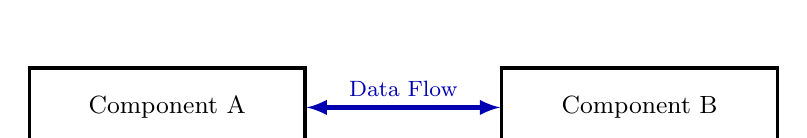
\begin{tikzpicture}[
        box/.style={rectangle, draw=black, very thick, minimum width=3.5cm, minimum height=1cm, align=center, fill=white, font=\small},
        arrow/.style={<->, very thick, >=latex}]

        \node[box] (A) at (0,0) {Component A};
        \node[box] (B) at (6,0) {Component B};

        \draw[arrow, blue!70!black, line width=1.5pt] (A.east) -- (B.west)
            node[midway, above, font=\footnotesize]{Data Flow};

    \end{tikzpicture}
    \caption{System Architecture Diagram}
\end{figure}

\subsection{Component Table}
\begin{table}[H]
    \centering
    \begin{tabularx}{\textwidth}{@{}lX@{}}
        \toprule
        \textbf{Component} & \textbf{Description} \\
        \midrule
        \texttt{component\_a.c} & Description of component A. \\
        \texttt{component\_b.c} & Description of component B. \\
        \bottomrule
    \end{tabularx}
    \caption{Component Overview}
\end{table}

\newpage

% ============================================================
% 3. SPECIFICATION
% ============================================================
\section{Specification}

\subsection{Format Overview}
Describe the data format or protocol specification here.

\begin{center}
    \begin{tabular}{|c|c|c|c|}
        \hline
        \textbf{Field A} & \textbf{Field B} & \textbf{Field C} & \textbf{CRC} \\
        4 bytes          & 2 bytes          & N bytes          & 2 bytes      \\
        \hline
    \end{tabular}
\end{center}

\subsection{Field Descriptions}
\begin{description}[style=nextline]
    \item[\textbf{Field A}] Description of Field A.
    \item[\textbf{Field B}] Description of Field B.
    \item[\textbf{Field C}] Description of Field C (variable length).
\end{description}

\newpage

% ============================================================
% 4. CODE EXAMPLES
% ============================================================
\section{Code Examples}

\subsection{Example Code}
\begin{lstlisting}[caption={Example C code snippet}]
#include <stdint.h>
#include <stdbool.h>

typedef struct {
    uint8_t  field_a;
    uint16_t field_b;
    uint32_t field_c;
} my_struct_t;

int my_function(my_struct_t *s) {
    if (s == NULL) return -1;
    s->field_a = 0x01;
    s->field_b = 0xABCD;
    return 0;
}
\end{lstlisting}

\newpage

% ============================================================
% 5. PERFORMANCE
% ============================================================
\section{Performance}

\begin{table}[H]
    \centering
    \begin{tabular}{@{}llll@{}}
        \toprule
        \textbf{Metric} & \textbf{Baseline} & \textbf{Optimized} & \textbf{Improvement} \\
        \midrule
        Metric A & 100 ms & 50 ms  & 2$\times$ faster \\
        Metric B & 200 kB & 40 kB  & 80\% reduction \\
        \bottomrule
    \end{tabular}
    \caption{Performance Summary}
\end{table}

\newpage

% ============================================================
% 6. SECURITY
% ============================================================
\section{Security Considerations}

\begin{alertbox}
    Describe any security considerations, threat models, or warnings relevant to your project here.
\end{alertbox}

\subsection{Threat Model}
Describe the threat model here.

\subsection{Mitigations}
\begin{itemize}[noitemsep]
    \item \textbf{Mitigation 1:} Description.
    \item \textbf{Mitigation 2:} Description.
\end{itemize}

\newpage

% ============================================================
% APPENDIX
% ============================================================
\appendix
\section{Appendix A: Glossary}

\begin{description}[style=nextline]
    \item[\textbf{Term 1}] Definition of term 1.
    \item[\textbf{Term 2}] Definition of term 2.
\end{description}

\section{Appendix B: References}
\begin{itemize}[noitemsep]
    \item Reference 1
    \item Reference 2
\end{itemize}

\end{document}
